\section{Combinatorial Analysis}
\section{Axioms}
There are two important rules in combinatorics: the rule of sum, and the rule of product.

The rule of sum says, if we have $a$ ways to finish a task using one method and alternatively, $b$ ways to finish the same task using another method, then there are $ab$ ways of finish this task. More generally,
\begin{equation}
	|S_1 \cup S_2 \cup \ldots \cup S_n| = |S_1| + |S_2| + \ldots + |S_n|
\end{equation}

One extension of the rule of sum is the inclusion-exclusion principle, which does not require sets $A_i$ to be disjoint. This does include the rule of sum, in that if sets $A_i$ are disjoint, the terms from the second to the last are all zero.
\begin{equation}
\begin{split}
|\bigcup_{i=1}^n A_i| = & \sum_{i=1}^n|A_i| - \sum_{1 \le i < j \le n}|A_i\cap A_j| + \sum_{1 \le i < j < k \le n}|A_i\cap A_j\cap A_k|-\ \cdots\ \\
&  +  \left(-1\right)^{n-1} |A_1\cap\cdots\cap A_n|
\end{split}
\end{equation}

The rule of product says, if finishing one task requires two steps, and there are $a$ ways to choose in the first step and $b$ ways to choose in the second step, then there are $ab$ ways to finish this task. More generally,
\begin{equation}
|S_1 \times S_2 \times \cdots \times S_n| = |S_{1}| \cdot |S_{2}| \cdots |S_{n}|
\end{equation}

\section{Binomial Coefficient and Its Applications}
\subsection{Binomial Coefficient}
We list here some of the useful binomial identities, all numbers are nature number (not including 0).

\begin{equation}
	{n \choose k} = {n \choose n-k}
\end{equation}

\begin{equation}\label{eq:subset_count}
	\sum^n_{k=0} {n \choose k} = 2^n
\end{equation}

\begin{equation}
	{n \choose k} = \frac{n}{k}{n-1 \choose k-1}
\end{equation}

\noindent{From the famous Pascal's rule,}
\begin{equation}\label{eq:Pascal's_rule}
	{n \choose k} + {n \choose k+1} = {n+1 \choose k+1}
\end{equation}
There is another form which is equivalent to equation \ref{eq:Pascal's_rule},
\begin{equation}
	{n \choose k} = {n-1 \choose k-1} + {n-1 \choose k}
\end{equation}

\noindent Here is an example that uses the {\em{logarithmic differentiation}}, $f' = f \dot [\ln(f)]'$.
\begin{equation}
	\frac{d}{dt} {t \choose k} = {t \choose k} \sum^{k-1}_{i=0} \frac{1}{t-i}
\end{equation}

\noindent A list of series that involves binomial coefficients,
\begin{eqnarray}
	\sum^n_{k=0} {n \choose k} = 2^n \\
	\sum^n_{k=0} k {n \choose k} = n 2^{n-1} \\
	\sum^n_{k=0} k^2 {n \choose k} = (n+n^2) 2^{n-2}
\end{eqnarray}
These can all be obtained by examining the function value or derivatives of the function $(1+x)^\alpha$, where $\alpha$ could be any real number, and $|x| < 1$.

There are some identities that could be proved using combinatorial analysis, such as {\em{double counting}}. Here is an example,
\begin{equation}\label{eq:double_count}
	\sum^n_{k=1} {n \choose k} {k \choose q} = 2^{n-q} {n \choose q}
\end{equation}
The left side of equation \ref{eq:double_count} counts the number of ways of selecting $k$ elements first, and then choosing $q$ elements from the resulting subset. These $q$ elements could be identical for different $k$. The right hand side of the equation says this is equivalent to first choosing $q$ elements directly from the set, and merging them into one of the $2^{n-q}$ subset of the set containing all but those selected $q$ elements.

Another example is,
\begin{equation}
	\sum^{n_1}_{m_1=0} {n_1 \choose m_1} {n_2 \choose m-m_1} = {n \choose m}
\end{equation}
This simply means choosing $m=m_1+m_2$ objects from a set of $n=n_1+n_2$ objects is equivalent to choosing $m_1$ objects from $n_1$ objects, and $m_2$ objects from $n_2$ objects.

Sometimes, knowing the bounds and asymptotic formulae could be helpful.
\begin{equation}
	\left(\frac{n}{k}\right)^k \le {n \choose k} \le {\frac{n^k}{k!}} \le \left(\frac{n \cdot e}{k}\right)^k
\end{equation}

\begin{equation}
	{2n \choose n} \sim \frac{4^n}{\sqrt{\pi n}}, \mbox{ as } n \rightarrow \infty
\end{equation}

\subsection{Bernoulli Distribution}
\subsection{The i.i.d. Case: Binomial Distribution}
\subsection{The Batch Mode Case: Hypergeometric Distribution}



\section{Multinomial Coefficient and Its Applications}

\subsection{Multinomial Coefficient}
The notion of {\em{multinomial coefficient}} is a generalization of binomial coefficient, which is defined in the multinomial theorem:
\begin{equation*}
	(x_1+x_2+\ldots+x_r)^n = \sum_{(n_1,\ldots,n_r):n_1+\ldots,n_r=n} {n \choose n_1,n_2,\ldots,n_r}x_1^{n_1}x_2^{n_2} \ldots x_r^{n_r}
\end{equation*}
We call $n \choose n_1,n_2,\ldots,n_r$ the multinomial coefficient.

\begin{prob}
	A set of $n$ distinct items is to be divided into $r$ distinct groups of respective sizes $n_1, n_2, \ldots, n_r$, where $\sum^r_{i=1} n_i = n$. How many different divisions are possible?
\end{prob}
Note that there are $n \choose n_1$ possible choices for the first group; for each choice of the first group there are $n \choose n-n_1$ possible choices for the second group; and so on. Hence it follows that there are
\begin{equation*}
\begin{split}
	& {n \choose n_1} {n-n_1 \choose n_2} \ldots {n-n_1-n_2- \ldots -n_{r-1} \choose n_r} \\
	& = \frac{n!}{(n-n_1)!n_1!} \frac{(n-n_1)!}{(n-n_1-n_2)!n_2!} \ldots \frac{(n-n_1-n_2- \ldots -n_{r-1}!}{(0)!n_r!} \\
	& = \frac{n!}{n_1!n_2! \ldots n_r!}
\end{split}
\end{equation*}
possible divisions.

Alternatively, we can first permute these $n$ items, where there are $n!$ such orderings. The first $n_1$ elements are assigned to group $1$, the next $n_2$ elements are assigned to group $2$, and so on. However, for example, keeping all but $n_i$ group fixed, this method would generate $n_i!$ equivalent divisions (note the order within a group does not matter). Therefore, we need to cancel out the equivalent-group effect by dividing $n_1!n_2! \ldots n_r!$. Finally, the multinomial coefficient is,
\begin{equation}
	{n \choose n_1,n_2,\ldots,n_r} = \frac{n!}{n_1!n_2! \ldots n_r!}
\end{equation}

\section{Categorical Distribution}
\section{Multinomial Distribution}


\section{Multiset Coefficient and Its Applications}
\subsection{Multiset Coefficient}
The notion of multiset (or bag) is a generalization of the notion of set in which members are allowed to appear more than once.

The number of times an element belongs to the multiset is the {\em{multiplicity}} of that member. The total number of elements in a multiset, including repeated memberships, is the {\em{cardinality}} of the multiset. For example, in the multiset \{a, a, b, b, b, c\} the multiplicities of the members a, b, and c are respectively 2, 3, and 1, and the cardinality of the multiset is 6.

The number of multisets of cardinality $k$, with elements taken from a finite set of cardinality $n$, is called the {\em{multiset}} coefficient or {\em{multiset number}}, and is denoted as $\left(\!\!{n\choose k}\!\!\right)$. It is equivalent to asking, with replacement, the number of all possible combinations of making $k$ draws from a urn with $n$ distinguishable balls labeled $1 \dots n$.

\begin{prob}\label{prob:multiset}
	With replacement, how many possible combinations to make $k$ draws from a urn with $n$ distinguishable balls labeled $1 \dots n$?
\end{prob}
%If we translate this prob directly to the combinatorial language, \smallmarginpar{It is NOT the sum of all the multinomial coefficients, which can be seen by computing $(1+ \dots +1)^k$, that is, $\sum {k \choose N_1, N_2, \ldots, N_n} = n^k$.} we may end up with counting the total number of the multinomial coefficients (actually, it is also correct). To solve this prob, let's first see a similar example.

\begin{prob}
	Suppose $k$ balls that are indistinguishable from each other are to be distributed into $n$ distinguishable (non-empty) urns, how many different outcomes are possible?
\end{prob}
%We note that this prob is equivalent to selecting $n-1$ of the $k-1$ spaces between (fixed) adjacent objects as our dividing points, \smallmarginpar{Objects being adjacent ensures the non-emptiness.} e.g., $OOO|OOO|OO$. We count the "bars" as urns (in total $n$) and big "O" as balls (in total $k$). Therefore, there are $k-1 \choose n-1$ such outcomes.\\


Now, we are ready to go back to our original prob. prob \ref{prob:multiset} could be asked this way: if however, we allow empty urns, how many outcomes are possible?

%One possible way of borrowing the non-empty case solution to solve the empty one is by starting with $k+n$ balls (instead of $k$), and place them into $n$ urns, \smallmarginpar{It is of probability 1 to remove one ball from each urn.} however at last remove one ball from each urn (so in total $n$). Because some of the urns may only contain one ball, this would give us the number of orderings $n+r-1 \choose r-1$. Another way to look at it is to allow all $k+n-1$ positions (not gaps) available to both symbols, and we count all balls between two bars the same type. Hence, the number of all possible combinations is ${n+k-1 \choose n-1} = {n+k-1 \choose k}$. Note, this scheme is allowing emptiness, because two ``bars'' can be adjacent to each other.

Another beautiful explanation is to construct an equivalent mapping. Note, the rule of drawing a series of $k$ numbers $a_1, a_2, \ldots, a_k$ from the set $\{1,2,\ldots,n\}$ with repetition is
\begin{equation*}
	1 \le a_1 \le a_2 \le \ldots \le a_k \le n
\end{equation*}
Now, a new series of $k$ numbers $b_1, b_2, \ldots, b_k$ can be constructed as follows
\begin{equation*}
\begin{aligned}
	1 \le a_1 & < & a_2+&1 < & \ldots & <  & a_k+&k-1 \le n+k-1 \\
	\downarrow & & \downarrow & & & & \downarrow \\
	b_1 & & b_2 & & \ldots & & b_k
\end{aligned}	
\end{equation*}
Note that $b_1 < b_2 < \ldots < b_k$. This is a model without replacement, and is a one-to-one mapping of the original prob. Under the model of drawing $k$ times from $n+k-1$ balls without replacement, the number of all possible combinations is $n+k-1 \choose k$, which is the same as what we obtained earlier.

A last thing worth noting is that, as we mentioned earlier, the number of all multinomial coefficients is also $k+n-1 \choose n-1$.

\section{Selected Topics}
\subsection{Double Factorial}
\subsection{Stirling Numbers}

\section{The Bertrand's Ballot prob}\label{chapter: Bertrand_Ballot_prob}
The Bertrand's ballot prob was first introduced by Joseph Bertrand in 1887, in the form of: "In an election where candidate A receives $p$ votes and candidate B receives $q$ votes with $p>q$, what is the probability that A will be strictly ahead of B throughout the count?"

%J. Bertrand himself gave the solution $\frac{p-q}{p+q}$  by using mathematical induction in the original paper. First of all, let's consider the initial case. At the first count, the vote can be either for candidate A or B. If it {\em{could}} \smallmarginpar{The word "could" means it is possible for an event to happen, but does not indicate its necessity.} be for candidate A, the simplest scenario is $p=1, q=0$, which is of probability 1 for candidate A to win the vote. This agrees with the formula. If it {\em{could}} be for candidate B, the simplest scenario is $p=2,q=1$, now there are ${2+1 \choose 1} = 3$ counting orders, i.e., AAB, ABA, or BAA. Note "AAA" is the only favorable order out of three possible orders. This again agrees with the formula. Assume the theorem is true when $p=a-1 \mbox{ and } q=b$ (last vote would be for candidate A), and when $p=a \mbox{ and } q=b-1$ (last vote would be for candidate B), which is the two possible scenarios at the second to last count. Now, considering the case with $p=a \mbox{ and } q=b$, the last vote is either for candidate A with probability $a/(a+b)$, or for candidate B with probability $b/(a+b)$. So the probability of candidate A to always lead the count is:

%\smallmarginpar{$\frac{(a-1)-b}{(a-1)+b} \mbox{ and } \frac{a-(b-1)}{a+(b-1)}$ are conditional probabilities, which are conditioned on the last count.}

\begin{equation*}
	\frac{a}{a+b} \frac{(a-1)-b}{(a-1)+b} + \frac{b}{a+b} \frac{a-(b-1)}{a+(b-1)} = \frac{a-b}{a+b}
\end{equation*}

This proves that the theorem is true for all $p>q\ge0$.

%D\'esir\'e Andr\'e in the same year gave an elegant proof of this prob, and the method is now called "the principle of reflection", or "the Andr\'e's reflection method", or "the Bertrand's ballot theorem". There are three facts need to noted. One is that, the sequences start with A or B with probability $p/(p+q)$ and $q/(p+q)$, respectively. The second fact is that, sequences start with B will for sure to tie at some point because A will finally win, and they are all unfavorable, because A already "loses" at the first count. The third is that, sequences that start with A can be classified into two cases, one is the case that A leads the counting process from beginning to the end which is the favorable case, the other is the case when the sequence will tie at some point which is the unfavorable case, importantly, the number of sequences in this latter case is the same as that of the sequences starting with B, because there is a bijection mapping. \smallmarginpar{One possible mapping is to denote the sequence as LBR, where "L" and "R" is the left and right part of the first tie position (must be a "B"), and then converting each character in L to its alternative, e.g., {\color{red}{AAB}}BABAA would become {\color{red}{BBA}}BABAA.} The probability is $1 - 2 \times \frac{q}{p+q} = \frac{p-q}{p+q}$.

The number of the unfavorable cases is $2 \times {p+q-1 \choose q-1}$, of which half starts with "A" and another half starts with "B", as explained above. The number of favorable cases is ${p+q-1 \choose p-1} - {p+q-1 \choose q-1}$. Actually, $\frac{{p+q-1 \choose p-1} - {p+q-1 \choose q-1}}{{p+q \choose p}} = \frac{p-q}{p+q}$.

Consider now the prob to find the probability that the second candidate is never ahead (i.e. ties are allowed); the solution is $\frac{p+1-q}{p+1}$. This is simply seen by awaring the following equivalent description:
\begin{itemize}
	\item same as the basic version, ties are NOT allowed; but,
	\item there are $p+1$ votes for candidate A and $q$ votes for candidate B;
	\item the first vote is for candidate A;
\end{itemize}
The probability can then be computed as:
\begin{equation*}
\begin{split}
	P(\mbox{A winning \mbox{\em{with}} ties}) & = P(\mbox{A winning \mbox{\em{without}} ties} \mid \mbox{the first vote is A})\\
	& =  \frac{P(\mbox{A winning without ties} \mbox{\em{ and }} \mbox{the first vote is A})}{P(\mbox{the first vote is A})}\\
	& = \frac{(p+1-q)/(p+1+q)}{(p+1)/(p+1+q)} = \frac{p+1-q}{p+1}
\end{split}
 \end{equation*}

 Another way to look at this prob is to model it as the following: represent a voting sequence as a lattice path on the Cartesian plane and,
\begin{itemize}
	\item Start the path at (0, 0);
	\item Each time a vote for the first candidate is received move right 1 unit;
	\item Each time a vote for the second candidate is received move up 1 unit.
\end{itemize}
Each such path corresponds to a unique sequence of votes and will end at $(p, q)$. A sequence is ``good'' exactly when the corresponding path never goes above the diagonal line $y = x$; equivalently, a sequence is ``bad'' exactly when the corresponding path touches the line $y = x + 1$. For each ``bad'' path P, define a new path P' by reflecting the part of P up to the first point it touches the line across it. P' is a path from (-1, 1) to (p, q). The same operation applied again restores the original P. This produces a one-to-one correspondence between the ``bad'' paths and the paths from (-1, 1) to (p, q). The number of these paths is $p+q \choose q-1$. So the probability asked is $\frac{{p+q \choose q} - {p+q \choose q-1}}{{p+q \choose p}} = \frac{p+1-q}{p+1}$.

%\begin{figure}[htb]
%	\centering	
%	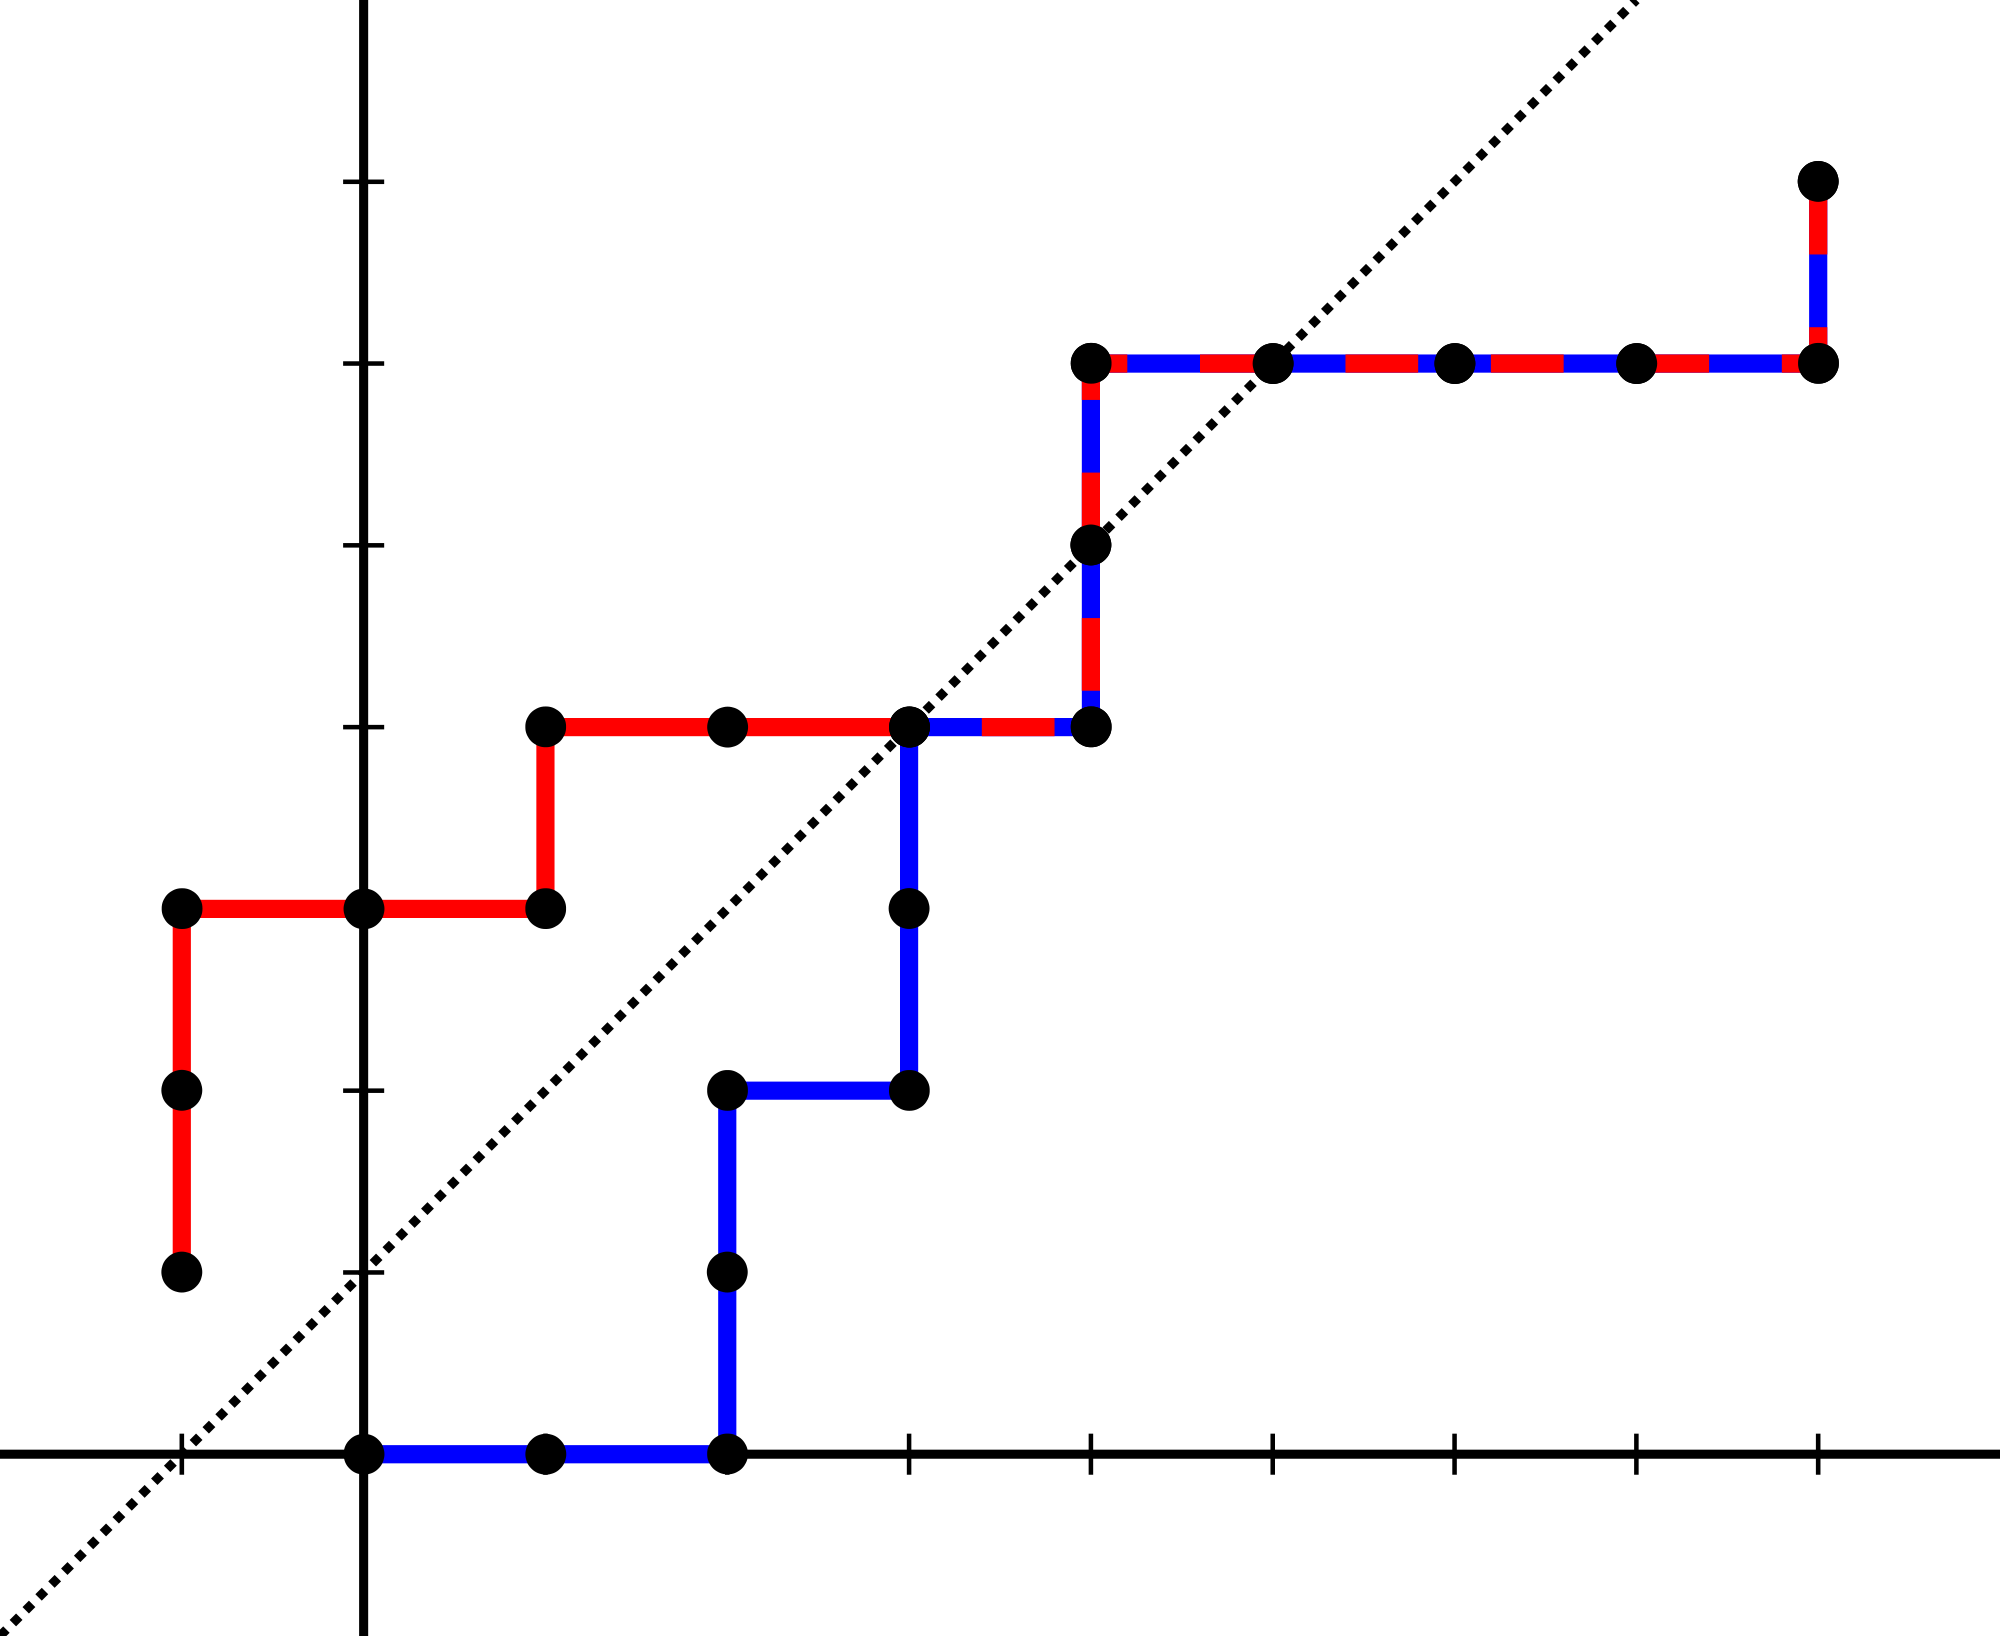
\includegraphics[width=150pt]{2000px-AndreReflection.png}
%	\caption{Bertrand's Ballot prob allowing Ties}
%	\label{fig:Bertrand's_Ballot_prob}
%\end{figure}

An interesting application of this is the famous Catalan number formula, which can be introduced under the random walk story. A random walk on the integers is to take $n$ steps of unit length, beginning at the origin and ending at the point $m$, that never become negative. Assuming $n$ and $m$ have the same parity and $n \ge m \ge 0$, this number is, according to the Bertrand's Ballot prob allowing ties,
\begin{equation*}
	{n \choose \frac{n+m}{2}} - {n \choose \frac{n+m}{2}+1} = \frac{m+1}{\frac{n+m}{2}+1} {n \choose \frac{n+m}{2}}
\end{equation*}
Here, $p+q=n$ and $p-q=m$, compared to our used settings. When $m=0$ and $n$ is even, this gives the Catalan number $\frac{1}{\frac{n}{2}+1} {n \choose \frac{n}{2}}$.

Let's tweak this prob a little bit more. Let's say candidate A starts at $a$ ``bonus'' votes, not 0. That is to say, the system goes from $(0,a)$ to $(p+q,p+a-q)$. If we do not allow ties, all paths hit the x-axis will be unfavorable, and the number of these paths equals the number of paths from $(0,a)$ to its ``mirror'' point $(p+q,-p-a+q)$. So, there are in total ${p+q \choose p+a}$ unfavorable paths, and the probability is $1 - \frac{{p+q \choose p+a}}{{p+q \choose p}}$. Note when $a=0$, there is already a tie, and the question really should be asked as: ``What if the first count is A, and then the process never has a tie''. So the probability should compute as:
\begin{equation*}
	1 - \frac{p}{p+q} \frac{{p-1+q \choose p-1}}{{p-1+q \choose p-1}} = \frac{p-q}{p+q}
\end{equation*}
It should have no prob with $a>0$.

If we allow ties, the ``mirror'' point should be reflected against $y=-1$, so it becomes $(p+q,-2-p-a+q)$. Now, suppose we go up $u$ steps and go down $d$ steps. Solving the following equations:
\begin{eqnarray*}
	u+d & = & p+q\\
	u+a-d & = & -2-p-a+q
\end{eqnarray*}
gives us $u=q-a-1$ and $d=p+a+1$. So there are ${p+q \choose p+a+1}$ paths unfavorable, and the probability is then $1-\frac{{p+q \choose p+a+1}}{{p+q \choose p}}$. When $a=0$, this becomes $\frac{p+1-q}{p+1}$, which agrees with what we obtained earlier.

In summary, if one starts at $(0,a)$ and ends at $(p+q,p+a-q)$, the number of unfavorable paths is $p+q \choose p+a$ if not allowing ties, $p+q \choose p+a+1$ if allowing ties.


\section{Catalan Number}
In chapter \ref{chapter: Bertrand_Ballot_prob}, we first met Catalan number from the generalized Bertrand's Ballot prob. We write here again the definition of Catalan number, with an intuitive interpretation.

The Catalan number is defined as,
\begin{equation}
	C_n = \frac{1}{n+1} {2n \choose n}
\end{equation}
The underlying story reads: Given two urns, one with $n$ red balls and the other with $n$ black balls, we want to draw one ball at a time (either red or black), such that at no time the number of pre-specified color is less than its alternative.

Since the Catalan number is associated with two equal-sized sets, it is oftentimes co-occurrent  with the words "pair", "full binary", and etc. 